\documentclass[a4paper,titlepage,11pt]{ltjsarticle}
\usepackage{graphicx}
\usepackage{color}
\usepackage{amssymb}
\usepackage{here}
\usepackage{listings}
\lstset{
	%プログラム言語(複数の言語に対応,C,C++も可)
 	language = C,
 	%背景色と透過度
 	backgroundcolor={\color[gray]{.90}},
 	%枠外に行った時の自動改行
 	breaklines = true,
 	%自動改行後のインデント量(デフォルトでは20[pt])	
 	breakindent = 9pt,
 	%標準の書体
 	basicstyle = \ttfamily\scriptsize\fontsize{8}{9},
 	%コメントの書体
 	commentstyle = {\itshape \color[cmyk]{1,0.4,1,0}},
 	%関数名等の色の設定
 	classoffset = 0,
 	%キーワード(int, ifなど)の書体
 	keywordstyle = {\bfseries \color[cmyk]{0,1,0,0}},
 	%表示する文字の書体
 	stringstyle = {\ttfamily \color[rgb]{0,0,1}},
 	%枠 "t"は上に線を記載, "T"は上に二重線を記載
	%他オプション:leftline,topline,bottomline,lines,single,shadowbox
 	frame = TBrl,
 	%frameまでの間隔(行番号とプログラムの間)
 	framesep = 5pt,
 	%行番号の位置
 	numbers = left,
	%行番号の間隔
 	stepnumber = 1,
	%行番号の書体
 	numberstyle = \tiny,
	%タブの大きさ
 	tabsize = 4,
 	%キャプションの場所("tb"ならば上下両方に記載)
 	captionpos = t
}
\begin{document}
%%タイトル
\title{情報システム工学実験Ⅰ 2023\\レポート}
\author{2022531033 22班 関川謙人}
\maketitle
\section{プログラムの概要}
\subsection{概要と目的}
課題8で制作したLEDを使ったラーメンタイマーを改良したプログラム。このタイマーは分単位での表記、操作ができるタイマーである。
\begin{itemize}
  \item 残り時間を分単位、秒単位に分けて測ることで残り時間をわかりやすくする。
  \item 一分調節すると,測る時間を60秒調節できる
\end{itemize}
以上の特徴により、秒単位だけで時間を測るタイマーよりわかりやすく、効率的に3分以内の時間を測ることを目的としている。
6つの赤LEDが秒単位を、2つの緑LEDが分単位を表記する。
\subsection{使用法}
始めに測る時間を指定する。この段階では、以下の操作ができる。
\begin{itemize}
  \item 上から2番目のボタンで1秒増やす。
  \item 上から3番目のボタンで1秒減らす。
  \item 下から3番目のボタンで1分増やす。
  \item 下から2番目のボタンで1分減らす。
  \item 一番下のボタンでタイマーをリセット、時間を0にする。
  \item 一番下のスタートボタンを押し、タイマーを作動させる。
\end{itemize}
以下の図はボタンとLEDの配置、役割、割り当てられたポートについて説明したものである。
\begin{figure}[H]
  \begin{center}
    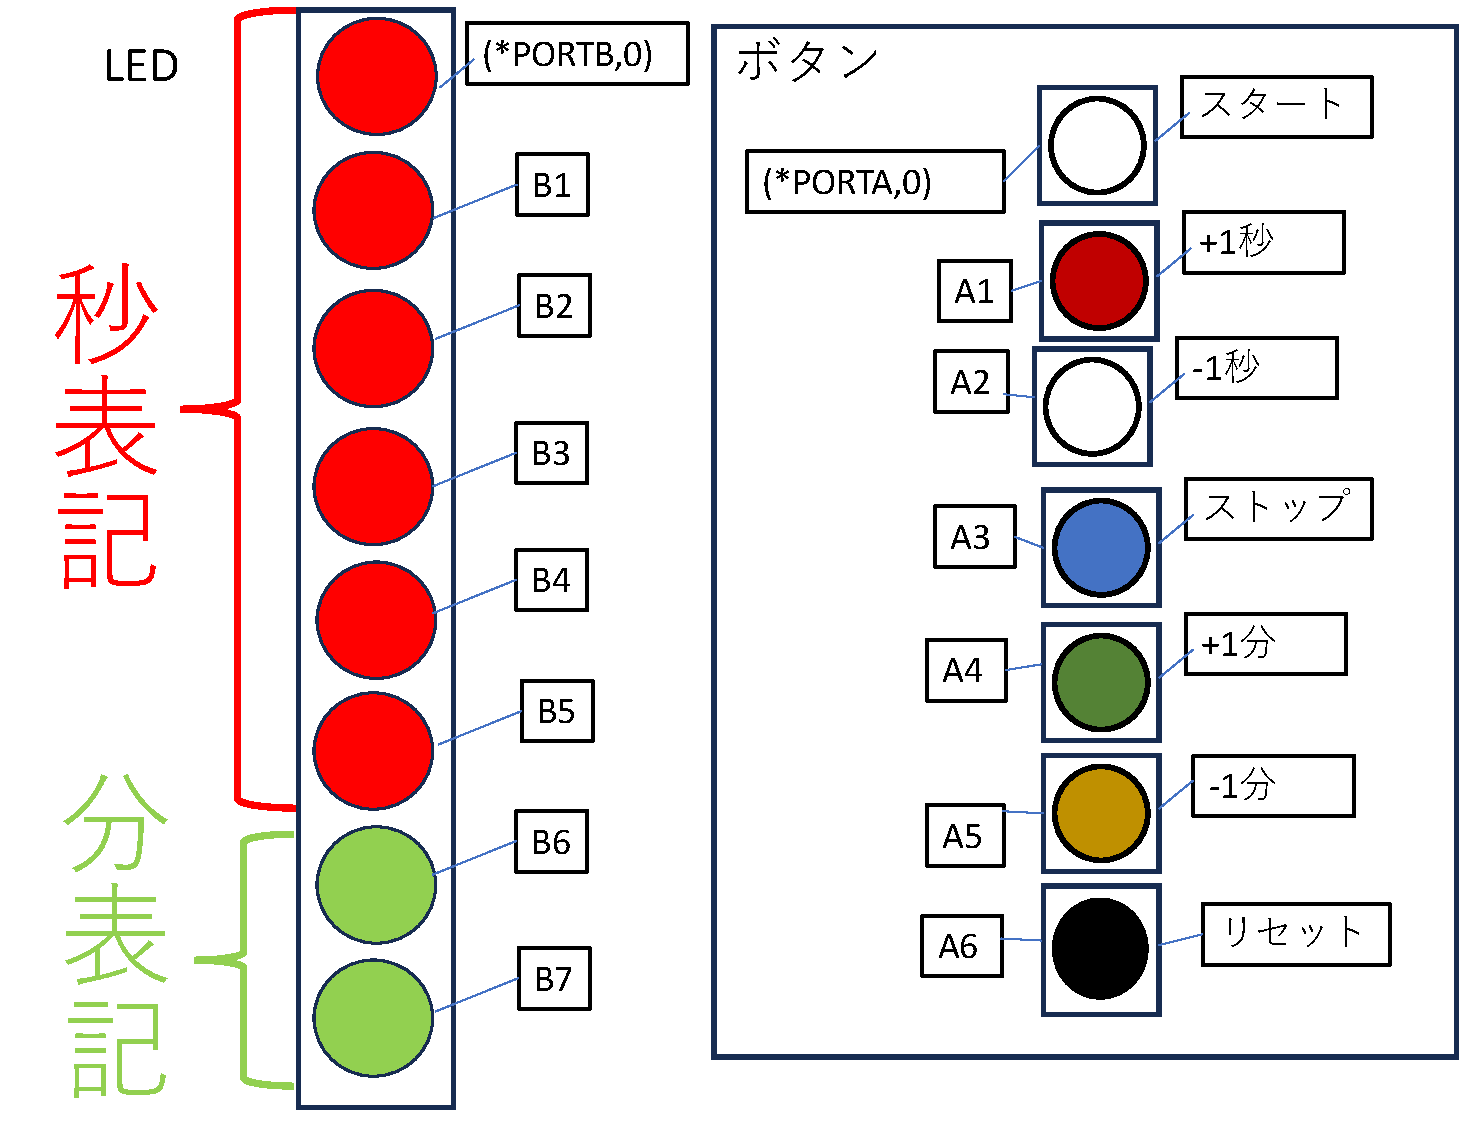
\includegraphics[width=100mm]{breadboard.pdf}
    \caption{ボタンとLEDの配置、役割}
  \end{center}
  \end{figure}

タイマーを作動させた後真ん中のストップボタンを押すと、タイマーが止まり時間指定を行う段階に戻る。

タイマーが時間を測り終わったとき、全てのLEDが1秒間隔で点滅する。時間指定を行う時、タイマーが作動している時の
両方において、LEDは残り時間を表す。
\section{プログラム作成の上での工夫、苦労}
オリジナルプログラムの作成はLEDの色を変え、分と秒を別々に表し、別々に操作できるように工夫した。それにはそこまで苦労しなかった。

課題をこなすのには苦労した。始めは容易に課題を解決できたので、ペアと別々にプログラムを組み一気に課題を進める計画を組んだが課題6で詰まってしまった。
具体的には、ボタンを押してもLEDの移り変わる速さが変わらない。その問題が解決してもLEDが一つの方向にしか動かないなどのエラーが起き、その問題がいつまでも
解決せず次に進めなかったのである。
原因はペアにプログラミングを任せたとき
\begin{itemize}
	\item 変数名を適当に付けてしまっていた。
	\item コメントを怠っていた
\end{itemize}
ことによってプログラムの流れが読みにくくなってしまったことである。
ペアと一緒にプログラムを組み、変数名やコメント、インデントなど打ち合わせをきちんとしながらプログラミングするべきであった。

このことから自らの能力を過信することの危険性、適切なコードを書くことの重要性、複数人で協力することでミスや見落としによるエラーを防げることを
身に染みて学んだ。自分がプログラミングを担当するときには以下の工夫をした。
\begin{itemize}
	\item 何を扱う変数かをわかりやすくするために変数名を独自に考える。
	\item コメントを使用してプログラムに細かく区切りをつける
\end{itemize}
これによってデバッグが簡単にできるように努めた。
\subsection{反省}
講義が終了した後に気付いた反省を以下に示す。
\begin{itemize}
  \item 時間を指定する段階のコードを先に配置すべきであった。
  \item 変数、コメントは工夫したが、インデントはできていなかった。
  \item 秒数の変数をcountではなくsecondにすべきであった
  \item 分数を減らす条件をcount=-1にする理由を理解せずにcount=-1に設定してしまった。
  \item 終了条件がなぜminute=-1なのかをコメントで説明していなかった。
	\item ストップボタンでのみタイマーを止める仕様にするつもりであったため、時間を調整するたびに変数trigの値を0にしてタイマーを止める必要性はなかった。
	\item ローカル関数を使用するのであれば、細かい処理をまとめてコードを読みやすくする形で使用するべきだった。
\end{itemize}
\section{ソースコード}
\subsection{ソースコードの補足説明}
終了条件がminute=-1となっているのは、終了条件をminute=0にするとminute=1からminute=0になるときに、時間を測り終わっていないのに
タイマーが終了してしまったからである。しかし一分減らす操作をタイマーを終了させる判定の後に置けば、終了条件をminute=0に設定しても
正常に動かせたのではないかと考えている。

また一分減らす時に秒数の残り時間を60秒でなく59秒にしている理由は、秒数のカウントを0-59秒の範囲で行っており、この時残り時間を60秒にしてしまうと
61秒カウントすることになってしまうからである。
\subsection{ソースコード}
制作したプログラムのソースコードを、以下に示す。
\lstinputlisting[caption = original.c ,label = オリジナルプログラム]{original.c}
\end{document}